\begin{center}
\textsc{\Large Laboratorio 7}~\\
\emph{\large Vídeo Juegos, Física en los Vídeo Juegos}
\end{center}

\section{Pre-Laboratorio}
\todo[inline]{Por hacer.}

\section{Introducción}
Para agregar realismo, nuevas mecánicas o mayor calidad visual se introducen leyes físicas dentro del motor de juego, es mayormente usado en juegos tridimensionales. Estas nuevos efectos se introducen en forma de simulaciones las cuales son aproximaciones de fenómenos reales utilizando valores discretos \cite{ian_gamephysics}.

\section{Simulaciones Físicas}
Hay dos clases centrales de simulaciones físicas, simulaciones de cuerpos rígidos (\emph{rigid-body physics}) y simulaciones de cuerpos blandos (\emph{soft-body physics}). En una simulación de cuerpos rígidos los objetos se agrupan entre categorías basadas en como deberían interaccionar, las simulaciones de cuerpos rígidos son menos intensas en cuanto a perdida de \emph{performance}. Las simulaciones de cuerpos blandos consisten en simular secciones individuales de cada objeto de tal forma que este se comporte de manera realista, usualmente utilizadas para simular objetos deformables como ropa o materiales destructibles \cite{ian_gamephysics}.
\begin{figure}[H]
\centering
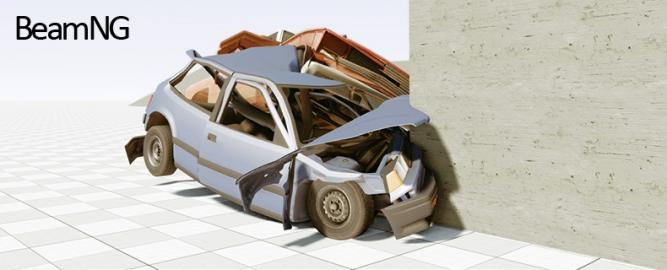
\includegraphics[width=0.9\linewidth]{semana7/beamng_gamephysics.jpg} 
\caption{BeamNG un video juego simulador de vehiculos que utiliza \emph{soft-body physics}.}
\end{figure}

\section{Sistemas de Partículas}
Es una técnica utilizada en físicas de juegos y computación gráfica en la que se usa una cantidad grande de pequeños \emph{sprites} u otros objetos visuales para simular ciertos fenómenos como sistemas altamente caoticos, fenomenos naturales o procesos causados por reacciones quimicas \cite{vanderburg_particlesystem}. 

Algunos ejemplos de fenómenos que son replicados utilizando sistemas de particulas, es el fuego, explosiones, humo, agua en movimiento (como cascadas de agua), nubes, estrellas, galaxias, etc. Es también común su uso para efectos visuales abstractos.
\begin{figure}[H]
\centering
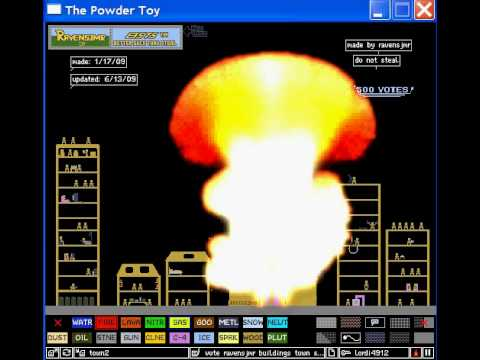
\includegraphics[width=0.9\linewidth]{semana7/powdertoy.jpg} 
\caption{Powder Toy un vídeo juego simulador de físicas 2D que utiliza sistemas de particulas para ciertas reacciones químicas.}
\end{figure}

\section{Físicas \emph{Ragdoll}}
Es una tecnica de simulacion que consiste en la animación procedimental de un personaje cuando este muere (u otro estado definido por el juego para causar \emph{ragdoll}, consiste en tratar a un objeto o personaje como una serie de objetos sólidos (huesos) conectados en distintos puntos formando un esqueleto. La simulación ocurre cuando el evento necesario para causar físicas \emph{ragdoll} sobre un objeto o personaje sucede, en los vídeo juegos esto pasa usualmente cuando el personaje muere \cite{eric_ragdoll}.

\section{Proyectiles}
En algunos vídeo juegos los objetos de tipo proyectil son sometidos a simulaciones físicas o aproximaciones. Usualmente en la programación de un juego un proyectil sigue una linea recta o parabólica y en caso de colisión se inicia algún evento. Otros juegos consideran factores que afectan la trayectoria del proyectil tales como resistencia y/o dirección al viento, velocidad de proyectil (en vez de una trayectoria inmediata el proyectil posee una velocidad en espacio), gravedad, entre otros \cite{fifa_physics}.

\begin{figure}[H]
\centering
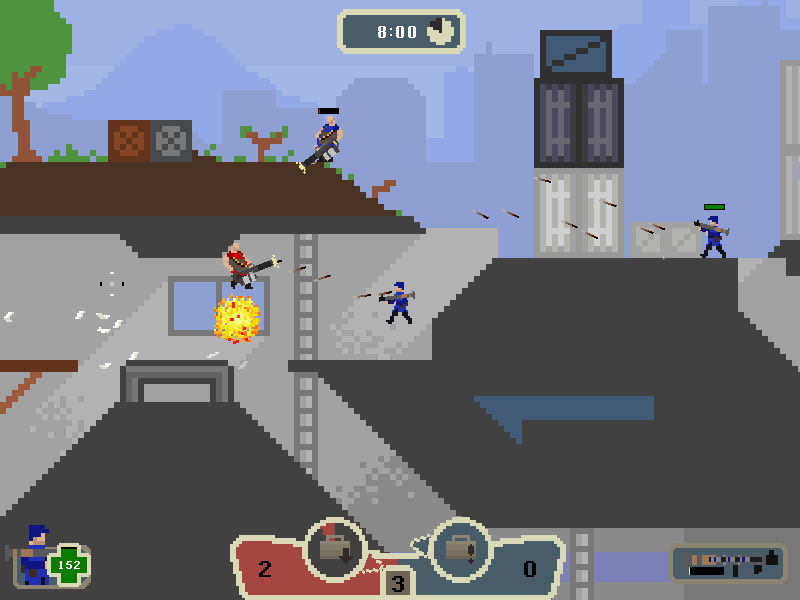
\includegraphics[width=0.9\linewidth]{semana7/Gang_Garrison_2.png} 
\caption{Gang Garrison 2 un shooter 2D basado en Team Fortress 2 un shooter 3D, distintas clases tienen distintos tipos de proyectiles.}
\end{figure}


\section{Actividad}
\todo[inline]{Por hacer.}